% This file was created by tikzplotlib v0.9.1.
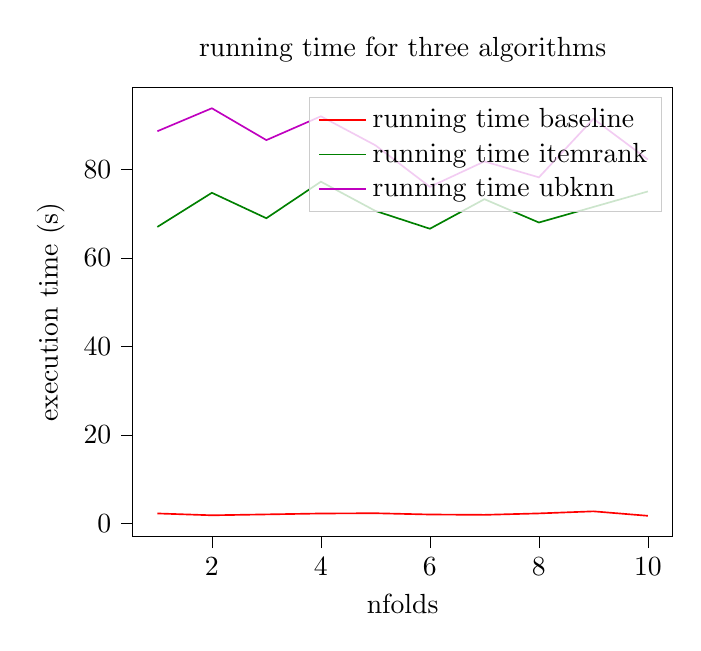
\begin{tikzpicture}

\definecolor{color0}{rgb}{0.75,0,0.75}

\begin{axis}[
legend cell align={left},
legend style={fill opacity=0.8, draw opacity=1, text opacity=1, draw=white!80!black},
tick align=outside,
tick pos=left,
title={running time for three algorithms},
x grid style={white!69.0196078431373!black},
xlabel={nfolds},
xmin=0.55, xmax=10.45,
xtick style={color=black},
y grid style={white!69.0196078431373!black},
ylabel={execution time (s)},
ymin=-2.85424687862396, ymax=98.4023158788681,
ytick style={color=black}
]
\addplot [semithick, red]
table {%
1 2.2828962802887
2 1.86600828170776
3 2.06847143173218
4 2.27491593360901
5 2.32877326011658
6 2.043536901474
7 1.9677300453186
8 2.29187321662903
9 2.76147627830505
10 1.7483241558075
};
\addlegendentry{running time baseline}
\addplot [semithick, green!50!black]
table {%
1 66.9989132881165
2 74.7070858478546
3 68.9600977897644
4 77.2165644168854
5 70.6155784130096
6 66.5847642421722
7 73.26203083992
8 67.9922344684601
9 71.5018441677094
10 75.0114684104919
};
\addlegendentry{running time itemrank}
\addplot [semithick, color0]
table {%
1 88.6110994815826
2 93.7997448444366
3 86.6055734157562
4 91.9813599586487
5 85.4344854354858
6 76.0483651161194
7 81.788341999054
8 78.1909592151642
9 91.4168260097504
10 82.2211849689484
};
\addlegendentry{running time ubknn}
\end{axis}

\end{tikzpicture}
